\PassOptionsToPackage{dvipdfmx}{graphicx}% NOTE: only for Japanese
\PassOptionsToPackage{dvipdfmx}{xcolor}% NOTE: only for Japanese
\documentclass[sip,biber]{now-journal}
\addbibresource{IEEEabrv.bib}
\addbibresource{ref.bib}

\usepackage[nolist,nohyperlinks]{acronym}
\usepackage{amsfonts}
\usepackage{bm}
\usepackage{mathtools}
\usepackage{interval}
\usepackage{siunitx}
\usepackage[skip=1pt]{subcaption}

% reload hyperref
\usepackage[colorlinks=true, allcolors=blue, plainpages=false, pdfpagelabels=true]{hyperref}
\usepackage{breakurl}

% cleveref setting
\usepackage[capitalise]{cleveref}
\crefformat{equation}{(#2#1#3)}
\Crefformat{equation}{#2Equation~(#1)#3}
\crefformat{section}{Section~#2#1{}#3}
\crefname{algorithm}{Algorithm}{Algorithms}
\crefname{equation}{}{}
\crefname{figure}{Figure}{Figures}
\crefname{section}{Section}{Sections}
\def\crefrangeconjunction{--}

% psuedo codes
\usepackage{xcolor}
\usepackage[theorems,skins]{tcolorbox}
\usepackage{tabularx}
\usepackage{pseudo}
\newtcbtheorem[crefname = {Algorithm}{algorithms}]{algorithm}{Algorithm}{pseudo/booktabs, float=t, theorem hanging indent=0pt}{alg}
\pseudodefinestyle{fullwidth}{
    begin-tabular=
    \tabularx{\textwidth}[t]{@{}
        r                                          % Labels
        >{\leavevmode\pseudosetup}                 % Indent, font, ...
        X                                          % Code (flexible)
        >{\leavevmode} % Comment styling
        p{0.20\textwidth}                           % Comments (fixed)
        @{}},
    end-tabular=\endtabularx,
}
\pseudoset{%
   fullwidth,
   kwfont=\sffamily\bfseries,
   font=\kwfont,
   prfont=\textsf,
   hsep=.3em,
   indent-mark,
   indent-mark-shift=.5em,
   indent-length=1em,
   line-height=1.5,
   ct-left=\hfill\texttt{//}~,
   ct-right=,
   % label=\textcircled{\ttfamily\scriptsize\arabic*},
   label=,
   % ref,
}

% Align euqality or replacement in pseudo codes
% ref: https://latex.org/forum/viewtopic.php?t=26363
\usepackage{xparse}
\DeclareDocumentCommand{\psm}{m O{$\gets$}}{% pseudocode-math
  {\hphantom{$W_{k,f,t - 1}$}\llap{#1}~#2}%
  % {\rlap{#1}\hphantom{$W_{k,f,t}$}#2}%
}

% Original style files
\usepackage{bsssym}
\newcommand{\todo}[1]{\textcolor{red}{#1}}

% Document information
\title{Self-Rotation-Robust Online Independent Vector Analysis with\\Sound Field Interpolation on Circular Microphone Array}
\fancyhead[LO]{\footnotesize\textit{Self-rotation-robust online independent vector analysis with sound field interpolation on circular microphone array}}
\author{Nakashima, Taishi}
\affil{Tokyo Metropolitan University, Tokyo, Japan}
\author{Wakabayashi, Yukoh}
\affil{Toyohashi University of Technology, Aichi, Japan}
\author[1]{Ono, Nobutaka}
\creditline{%
  Corresponding author: Taishi Nakashima, \href{mailto:taishi@ieee.org}{taishi@ieee.org}.
  This work was supported by JSPS KAKENHI Grant Number 21J22039 and JST CREST Grant Number JPMJCR19A3.
}

\articledatabox{
  Received XX June 2023; Revised YY Sep 2023
  ISSN XXXX-YYYY; DOI xx.yyyy/zzz.wwwwwwww\\
  \copyright 2023 T. Nakashima, Y. Wakabayashi, and N. Ono
}

\keywords{
  Blind source separation,
  online independent vector analysis,
  circular microphone array,
  sound field interpolation
}

\begin{document}

\begin{abstract}
  % 本論文では,マイクロホンアレイの回転に頑健なオンラインブラインド音源分離手法を提案する.
  % Online auxiliary-function-based independent vector analysis (OIVA)はリアルタイムBSSを実現するための有望な手法のひとつである.
  % リアルタイムBSSを実用化するためには,音源やマイクの移動といった環境の変化に対する頑健性が重要な課題である.
  % 一般的にリアルタイム処理の最中に環境の変化が起こった場合はパラメータの再推定が必要である.
  % OIVAでは音源のなめらかな移動に対して頑健かつ高い分離性能を獲得できることが示されていた.
  % しかし,OIVAはマイクの突発的な移動に対しては十分な性能が得られない.
  % そこで本論文では,円状等間隔マイクロホンアレイ(CMA)のための音場補間処理を利用したOIVAを提案する.
  % 音場補間はCMAの回転を打ち消し,パラメータの再推定を必要とせずにBSSを可能にする.
  % シミュレーション実験の結果は音場補間によりマイクが回転する状況における音源分離の頑健性が向上したことを確認した.
  In this paper, we propose a robust online blind source separation (BSS) method against the self-rotation of microphone arrays.
  Online auxiliary-function-based independent vector analysis (OIVA) is one of the promising methods for real-time BSS.
  One major issue for real-time BSS is robustness against environmental changes such as the movement of the source or microphone.
  Parameter re-estimation is generally necessary if environmental changes occur during real-time processing.
  OIVA is robust against smooth movement of sources and achieves high separation performance.
  However, OIVA does not perform well against rapid movements of microphones.
  Therefore, we employ sound field interpolation (SFI) for circular microphone arrays (CMAs) with OIVA in this paper.
  SFI cancels out the rotation of the CMA, enabling us to apply BSS without parameter re-estimation.
  Simulation experiments confirmed that SFI improves the robustness of the OIVA in situations where the microphone is rotating.
\end{abstract}

\section{Introduction}\label{sec:intro}
% ブラインド音源分離は混合信号から目的の信号を分離する技術である.
% BSSの手法はIVAやその拡張などが有名である.
% これらの手法はすべて時不変な系を仮定している.
% それに対して,実応用のためにはマイクロホンや音源の移動など系の時間変化を考慮する必要がある.
% 系の時間変化を考慮するためには,信号を短いブロックに分割し,各ブロックに対してIVAを適用するやり方が考えられる.
% ブロックバッチの手法やオンラインの手法が考えられる.
%
% オンライン独立ベクトル分析は実時間で動作し,高い性能を示した.
% オンラインAuxIVA は補聴器への応用,残響除去との組み合わせ,高速なステアリングベクトル更新など最近活発に研究されている.
% オンラインAuxIVA ではフレームごとに分離行列を推定し,音響伝達系のゆるやかな時間変化に対応できる.
% しかし,新たな音源の出現やマイクの移動など,音響伝達系の突発的な変化が起こった場合には推定が難しくなり性能が著しく低下する.
%
% 音響伝達系の突発的な変化に対応するための音響信号処理手法がいくつか提案されている.
% 円状等間隔マイクロホンアレイ(circular microphone array; CMA)の回転を考え,音場の補間により対応する手法が提案されている.
% この手法はCMAの対称性を利用することで,CMAが回転する前の音場を簡単な線形演算により推定する.
% また,ビームフォーミング \cite{Wakabayashi:2021:ICASSP} やステアリングベクトル推定 \cite{Wakabayashi:2021:ASJ:A} への応用や,
% CMAの回転角度を自己推定する手法 \cite{Lian:2021:APSIPA} も提案されている.
% そこで,本稿では,CMAが回転する状況下のブラインド音源分離に取り組む.
% 音場補間によりCMAの回転の影響を打ち消しながらオンラインでブラインド音源分離処理を行う.
Blind source separation (BSS) \cite{Makino:2018:ASS} is a technique to extract the source signals from their observed mixture.
Popular approaches for BSS include independent vector analysis (IVA) \cite{Kim:2006:ASLP,Hiroe:2006:ICA} and extensions \cite{Kitamura:2016:ASLP,Nugraha:2020:SPL,Brendel:2020:SP}.
These methods assume a time-invariant acoustic transfer system (ATS).
On the other hand, for practical applications, it is necessary to consider time variations of the ATS, such as movements of the microphone or source.
Many methods have been proposed based on block batch \cite{Koldovsky:2019:ICASSP,Koldovsky:2021:SP,Jansky:2022:ASMP} or online processing \cite{Kim:2010:CASI,Taniguchi:2014:HSCMA}.

Online AuxIVA shows high separation performance in real-time situations \cite{Taniguchi:2014:HSCMA}.
It also has been actively researched recently for applications in hearing aids \cite{Sunohara:2017:ICASSP}, joint optimization with dereverberation \cite{Ueda:2021:ICASSP}, and computationally efficient optimization \cite{Nakashima:2023:ICASSP}.
Online AuxIVA estimates demixing matrices frame-by-frame manner and can track smooth environmental changes in ATS, such as slow movement of sources.
However, rapid changes in ATS, such as the emergence of new sources or microphone movement, makes online BSS difficult and thus degrade separation performance.

\todo{AR, VR関連のサーベイ追加}

Several methods have been proposed to cope with such rapid changes in ATS.
Sound field interpolation (SFI) for circular microphone array (CMA) has been proposed to address the rotation of a CMA \cite{Wakabayashi:2023:ASLP}.
This method exploits the symmetry of the CMA to estimate the sound field before the rotation of the CMA by a simple linear operation.
Applications to beamforming \cite{Wakabayashi:2021:ICASSP} and steering vector estimation \cite{Wakabayashi:2021:ASJ:A} have also been proposed,
as well as a method for self-estimating the rotation angle of a CMA \cite{Lian:2021:APSIPA}.

In this paper, we address blind source separation in situations where a CMA rotates.
SFT cancels out the effect of the rotation, and BSS is applied in the latter stage.
As described in \cref{sec:proposed}, simply applying SFI to online BSS is computationally expensive since SFI is required for the observed signal every time frame.
In contrast, this study introduces a more straightforward method than that and demonstrates its effectiveness through experiments.
Experiments show that our proposed scheme is significantly better than the conventional online AuxIVA for the source separation task.

The rest of this paper is organized as follows.
We formulate our motivation in \cref{sec:problem}.
\Cref{sec:conventional} describes SFI and how to apply it to online BSS.
In \cref{sec:proposed}, we propose an efficient online BSS that utilizes the information before and after the rotation of CMA.
We conduct some experiments to show the efficacy of the SFI for online BSS in \cref{sec:experiment}.
Finally, \cref{sec:conclusion} concludes this paper.

\section{Problem Formulation}\label{sec:problem}
% TODO: マイクが回転する状況での音源分離の図
We model the observed signal recorded with a circular microphone array (CMA) that may be rotated during processing.
Let $\Src$ and $\Mic$ be the number of sources and microphones, respectively.
We assume that the observed signal $\Obs _{\ft}$ is modeled as
\begin{equation}
  \Obs _{\ft} = \steer _{1,\ft} \sig _{1,\ft} + \dots + \steer _{\Src,\ft} \sig _{\Src,\ft} = \sum _{\src=1} ^{\Src} \steer _{\src,\ft} \sig _{\src,\ft},\label{eq:mix}
\end{equation}
in the short-time Fourier transform (STFT) domain,
where $\freq = 1, \dots, \Freq$ denotes the frequency bin index,
$\tframe = 1, \dots, \Tframe$ denotes the time frame index,
$\sig _{\src,\ft} \in \C\; (\src = 1, \dots, \Src)$ denotes the $\src$th source signal,
and $\steer _{\src,\ft} \in \C ^{\Mic}$ denotes the steering vector of the $\src$th source signal to each microphone.
Also, we here set the \emph{reference microphone} $\refmic = 1$ without loss of generality.
In this case, each steering vector can be denoted as
\begin{equation}
  \steer _{\src,\ft} \coloneqq \begin{bmatrix} 1 & \str _{2\src,\ft} & \dots & \str _{\Mic\src,\ft} \end{bmatrix} ^{\top}\; (\src = 1, \dots, \Src).
\end{equation}
In other words, $\str _{\mic\src,\ft} \; (\mic = 2, \dots, \Mic,\; \forall \src = 1, \dots, \Src)$ corresponds to the relative transfer function from the $\src$th source to the $\mic$th microphone.
Note that many BSS methods require a time-invariant mixing system $\steer _{\src,\freq}\; (\forall \src)$,
whereas, in this paper, steering vectors are time-variant $\steer _{\src,\ft}\; (\forall \src)$ to account for CMA rotations.
We aim to estimate \emph{source images} at the reference microphone $\sig _{1,\ft},\, \dots,\, \sig _{\Src,\ft}$, even if the CMA is rotated.

Next, we consider an online BSS problem with the model defined above.
We henceforth assume that the number of microphones of CMA is equal to that of sources; $\Mic = \Src$.
\renewcommand{\Mic}{\Src}%
We aim to estimate demixing matrices and estimated signals using only the current and past observed signals $\Obs _{\freq,1},\, \dots,\, \Obs _{\freq,\tframe}$:
\begin{align}
  \Demix _{\ft} &= \begin{bmatrix} \demix _{1\ft} & \dots & \demix _{\Src,\ft} \end{bmatrix} ^{\hermite} \in \C ^{\Src \times \Mic}, \\
  \Est _{\ft} &= \Demix _{\ft} \Obs _{\ft} \in \C ^{\Src},
\end{align}
where $\Demix _{\ft}$ is the demixing matrix, and $\Est _{\ft}$ is the estimated signal.

Unless specified, indices $\freq,\, \tframe,$ and $\src$ always ranges from 1 to $\Freq, \Tframe,$ and $\Src$, respectively.
We omit the bounds of sets over these indices when they span the ranges.
${\{\Obs _{\ft}\}}_{\ft}$ denotes the set of $\Obs _{\ft}$ for all $\freq$ and $\tframe$, for example.
\Cref{tab:notations} summarises the notations used in this paper.
\begin{table}[t]
  \centering
  \caption{Notations}\label{tab:notations}
  \begin{tabular}{lll}
    \toprule
      Symbol & Domain & Description \\
    \midrule
      % $\Mic$               & $\Z$                     & Number of microphones \\
      $\Src$                               & $\Z$                     & Number of sources \\
      $\steer _{\src,\ft}$                 & $\C ^{\Mic}$             & Steering vector \\
      $\sig _{\src,\ft}$                   & $\C$                     & Source signal \\
      $\Obs _{\ft}$                        & $\C^{\Mic}$              & Observed signal \\
      $\Demix _{\ft}$                      & $\C^{\Src \times \Mic}$  & Demixing matrix \\
      $\Est _{\ft}$                        & $\C^{\Mic}$              & Estimated signal \\
      $\cov _{\src,\ft}$                   & $\C^{\Mic \times \Mic}$  & Covariance matrix \\
      $\forget$                            & $\{\forget \in \R \mid 0 \leq \forget < 1\}$   & Forgetting factor \\
      $\rotSpat _{\tframe}$                & $\R$                     & Spatial rotation angle \\
      $\rotSmpl$                           & $\R$                     & Rotation angle coefficient on CMA \\
      $\rotFra$                            & $\R$                     & Rotation time \\
      $\rotMat (\rotSpat _{\tframe})$      & $\R ^{\Mic \times \Mic}$ & Rotation matrix \\
      $\refpos{\Obs} _{\ft}$ & $\C^{\Mic}$ & Observes signal at \textcolor{red}{\textbf{reference position}} \\
    \bottomrule
  \end{tabular}
\end{table}

\section{Conventional Methods}\label{sec:conventional}

\subsection{Online Auxiliary-Function-Based Independent Vector Analysis}\label{subsec:oiva}

Online AuxIVA \cite{Taniguchi:2014:HSCMA} is an online extension of AuxIVA \cite{Ono:2011:WASPAA} and estimates demixing matrices $\{\Demix _{\ft}\} _{\freq}$ at time frame $\tframe$ by minimizing the following objective function:
\begin{align}
  J _{\tframe}(\Demix _{\ft}) &= \sum _{\src = 1} ^{\Src} \demix _{\src,\ft} ^{\hermite} \cov _{\src,\ft} \demix _{\src,\ft} ^{\nohermite} - \logdet{\Demix _{\ft}} ^2, \label{eq:obj} \\
  \cov _{\src,\ft} &= \forget \cov _{\src,\ft[-1]} + (1 - \forget) \weight(\var _{\src,\tframe}) \Obs _{\ft} ^{\nohermite} \Obs _{\ft} ^{\hermite}, \label{eq:cov} \\
  \var _{\src,\tframe} &= \sqrt{\sum _{\freq=1} ^{\Freq} \lvert \demix ^{\hermite} _{\src,\ft} \Obs ^{\nohermite}_{\ft} \rvert ^2},
\end{align}
where $\weight\colon \R _{>0} \to \R _{>0}$ is defined as $\weight(\var) = \cont ' (\var) / 2 \var$ ($\cont '(\var)$ denotes the first derivative of $\cont (\var)$ with respect to $\var$),
$\cont(\var)$ is called a contrast function and derived from the probability density function of source signals,
and $\forget\; (0 \leq \forget < 1)$ is called a forgetting factor.
In this paper, we assume that $\weight (\var) = \Freq/{\var ^2}$, which represents the time-varying Gaussian distribution \cite{Ono:2012:APSIPA}.
Using the recursive update for covariance matrix \eqref{eq:cov}, we can apply efficient update methods proposed for batch AuxIVA algorithms, such as \emph{iterative projection (IP)} \cite{Ono:2011:WASPAA}, to minimize the objective function \eqref{eq:obj}.
IP cyclically updates each \emph{demixing vector} $\demix _{\src,\ft} ^{\hermite}\; (\src = 1, \dots, \Src)$ (row of the demixing matrix $\Demix _{\ft}$) using the following update rule:
\begin{align}
  \demix _{\src,\ft} &\gets (\Demix _{\ft} \cov _{\src\ft}) ^{-1} \eye _{\src} \label{eq:ip:proj}, \\
  \demix _{\src,\ft} &\gets \frac{{\demix _{\src,\ft}}}{{\sqrt{\demix _{\src,\ft} ^{\hermite} \cov _{\src,\ft} \demix _{\src,\ft}}}} \label{eq:ip:norm},
\end{align}
where $\eye _{\src} \in \R ^{\Src}$ is the canonical basis vector with the $\src$th element unity.
\Cref{alg:naive} summarises the Online AuxIVA algorithm.
\begin{algorithm}{Online AuxIVA (OIVA)}{naive}
  \textbf{Input:} $\{\Obs _{\ft}\} _{\freq},\, \{\Demix _{\ft[-1]}\}_{\freq},\, \{\cov _{\src,\ft[-1]}\}_{\src,\freq}$\\
  % \textbf{Output:} $\Est _{\ft},\, \Demix _{\ft},\, \cov _{\src,\ft}\; (\forall \src,\freq)$
  \textbf{Output:} $\{\Demix _{\ft}\}_{\freq},\, \{\cov _{\src,\ft}\}_{\src,\freq}$
  \begin{pseudo}
    {$\Demix _{\ft}$} $\gets$ $\Demix _{\ft[-1]}$ \ct{$(\forall \freq)$} \\
    for $\itr = 1,\, \dots,\, \Itr$ \\+
      for $\src = 1,\, \dots,\, \Src$ \\+
        {$\var _{\src,\tframe}$} $\gets$ $\sqrt{\sum _{\freq} \abs{\demix _{\src,\ft} ^{\hermite} \Obs _{\ft}} ^2}$ \\
        {$\cov _{\src,\ft}    $} $\gets$ $\forget \cov _{\src,\ft[-1]} + (1 - \forget) \weight(\var _{\src,\tframe}) \Obs _{\ft} \Obs _{\ft} ^{\hermite}$ \ct{$(\forall \freq)$}\\-
      forall $\src = 1, \dots, \Src$ \\+
        {$\demix _{\src,\ft}$} $\gets$ $\left(\Demix _{\ft} \cov _{\src,\ft}\right) ^{-1} \eye _{\src}$ \ct{$(\forall \freq)$}\\
        {$\demix _{\src,\ft}$} $\gets$ $\dfrac{\demix _{\src,\ft}}{\sqrt{\demix _{\src,\ft} ^{\hermite} \cov _{\src,\ft} \demix _{\src,\ft}}}$ \ct{$(\forall \freq)$}
        % {$\Est _{\ft}  $} $\gets$ $\Demix _{\ft} \Obs _{\ft}$ \ct{$(\forall \freq)$}
  \end{pseudo}
\end{algorithm}

\subsection{Sound Field Interpolation on Circular Microphone Array}
This subsection briefly reviews the sound field interpolation method on circular microphone array (CMA), which is originally proposed in \cite{Wakabayashi:2021:ICASSP}.
Let $\sfcma (\rotCoor)$ be a continuous sound pressure on the circumference of a circle at a spatial angle $\rotCoor \in \interval[open right,soft open fences]{0}{2\pi}$, as shown in \cref{fig:sfi}.
Then we observe a sound field with $\Mic$ microphones on the circle at even intervals.
The $\mic$th observed signal is denoted as
\begin{equation}
  \sfcma _{\mic} = \sfcma \left(2\pi \frac{\mic}{\Mic}\right),\; (\mic = 0, \dots, \Mic - 1).%
  \label{eq:sfi:model}
\end{equation}
In other words, we regard observations of the sound field with a CMA as discretizations of that along an angle on the circumference $\rotCoor$.
\begin{figure}[t]
  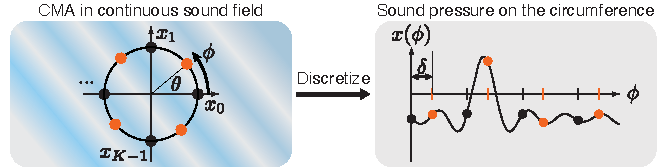
\includegraphics{figures/diagrams/sfi.pdf}
  \caption{%
    Concept of sound field interpolation on a circular microphone array.
    The left figure depicts the microphone array in a continuous sound field (six microphones in this example).
    Each black circle is a microphone at the reference position, and each gray cross is a microphone at the rotated position.
    Background colors indicate the sound pressure of a plane wave.
    The right figure depicts the sound pressure along the circumference.
  }%
  \label{fig:sfi}
\end{figure}

Next, we formulate a sound field interpolation problem with the model above.
If the CMA is rotated by a spatial angle $\rotSpat \in \R$, we can regard its observation as the $\rotSmpl$-sample shift of $\sfcma _{\mic}$;
\begin{equation}
  \sfcma \left(\frac{2\pi}{\Mic} \mic + \rotSpat \right)%
  \coloneqq
  \sfcma _{\mic + \rotSmpl},
  \label{eq:sfi:shift:obs}
\end{equation}
where $\rotSmpl = \frac{\Mic}{2\pi} \rotSpat$.
Also, we assume the \emph{``non-integer sample shift theorem''};
\begin{align}
  \dft _{\Src} [\sfcma _{\mic + \rotSmpl}] &= \Sfcma _{\src} \twid ^{\rotSmpl \src},%
  \label{eq:sfi:shift:dft}\\
  \twid &\coloneqq \exp \left(j\frac{2\pi}{\Mic}\right),
\end{align}
where $\dft _{\Src} [\sfcma _{\mic}]$ is the $\Mic$-points discrete Fourier transform (DFT) defined as
\begin{align}
  \dft _{\Src} [\sfcma _{\mic}] &= \sum _{\mic = 0} ^{\Mic - 1} \sfcma _{\mic} \twid ^{-\mic\src} \coloneqq \Sfcma _{\src},
  \intertext{and its inverse transform is defined as}
  \dft _{\Src} ^{-1} [\Sfcma _{\src}] &= \frac{1}{\Mic} \sum _{\src = 0} ^{\Mic - 1} \Sfcma _{\src} \twid ^{\mic\src}.
\end{align}
% and $j$ is the imaginary unit.
From these assumptions, we have
\begin{align}
  \sfcma _{\mic + \rotSmpl} &= \dft _{\Src} ^{-1} \left[\Sfcma _{\src} \twid ^{\rotSmpl \src}\right], \\
                            &= \frac{1}{\Mic} \sum _{\src \in \SRC} \left(\Sfcma _{\src}\twid ^{\rotSmpl\src} \right) \twid ^{\mic\src}, \\
                            &= \frac{1}{\Mic} \sum _{\src \in \SRC} \left(\sum _{n=0} ^{\Mic - 1} \sfcma _{n} \twid ^{-n\src}\right) \left( \twid ^{(\rotSmpl + \mic)\src} \right), \\
                            &= \sum _{\dum = 0} ^{\Mic - 1} \sfcma _{\dum} \left( \frac{1}{\Mic} \sum _{\src \in \SRC} \twid ^{(\rotSmpl + \mic - \dum)\src} \right)
                            \coloneqq \sum _{\dum = 0} ^{\Mic - 1} \sfcma _{\dum} \rotmat _{\mic, \dum}(\rotSmpl) \label{eq:sfi:elem},
\end{align}
where $\SRC$ is a set of indices defined as {\small\todo{(和の範囲を次のようにとる理由…?)}}
\begin{align}
  \SRC &= \left\{\left\lceil - \frac{\Mic-1}{2} \right\rceil, \dots, \left\lceil \frac{\Mic-1}{2} \right\rceil\right\} \\
       &=
  \begin{cases}
    \left\{-\frac{\Src}{2} + 1, -\frac{\Src}{2} + 2, \dots, \frac{\Src}{2}\right\} & \text{($\Src$ is even)} \\
    \left\{-\frac{\Src - 1}{2}, -\frac{\Src - 1}{2} + 1, \dots, \frac{\Src - 1}{2}\right\} & \text{($\Src$ is odd)}
  \end{cases}
\end{align}
The coefficient $\rotmat _{\mic,\dum}(\rotSmpl)$ can be calculated as
\begin{align}
  \rotmat _{\mic,\dum}(\rotSpat)
  &=
    \begin{cases}
      \displaystyle\frac{\twid ^{- \rotIdx (\frac{\Mic}{2} - 1) }}{\Mic} \frac{1 - \twid ^{\rotIdx \Mic}}{1 - \twid ^{\rotIdx}} & (\text{$\Mic$ is even}),\\[1em]
      \displaystyle\frac{\twid ^{- \rotIdx \frac{(\Src - 1)}{2}}}{\Mic} \frac{1 - \twid ^{\rotIdx \Mic}}{1 - \twid ^{\rotIdx}} & (\text{$\Mic$ is odd}),
    \end{cases}\label{eq:rot:twid} \\
  &=
    \begin{cases}
      \displaystyle \frac{\sinc{(\rotIdx)}}{\sinc{\left(\rotIdx / \Mic\right)}} \twid ^{\frac{\rotIdx}{2}} & (\text{$\Mic$ is even}),\\[1em]
      \displaystyle \frac{\sinc{(\rotIdx)}}{\sinc{\left(\rotIdx / \Mic\right)}} & (\text{$\Mic$ is odd}),
    \end{cases}\label{eq:rot:sinc}
\end{align}
where and $\rotIdx =\rotSmpl + \mic - \dum; (\mic, \dum = 0, \dots, \Mic - 1)$ \cite{Wakabayashi:2023:ASLP}.
Equations \eqref{eq:rot:twid} and \eqref{eq:rot:sinc} are alternative expressions for (3) in \cite{Wakabayashi:2023:ASLP}.
See Section II of \cite{Wakabayashi:2023:ASLP} for the detailed derivation.

The above relationship also holds in the frequency domain.
Let us define the following vector:
\begin{align}
  \bm{\sfcma} &= \begin{bmatrix} \sfcma _{0} & \dots & \sfcma _{\Mic - 1} \end{bmatrix} ^{\top}, \\
  \bm{\sfcma} _{\rotSmpl} &= \begin{bmatrix} \sfcma _{0+\rotSmpl} & \dots & \sfcma _{(\Mic - 1)+\rotSmpl} \end{bmatrix} ^{\top}.
\end{align}
From \eqref{eq:sfi:elem}, we have
\begin{equation}
  \bm{\sfcma} _{\rotSmpl}
  =
  \begin{bmatrix}
    \rotmat _{0, 0}(\rotSpat) & \dots & \rotmat _{0, \Mic - 1}(\rotSpat) \\
    \vdots & \ddots & \vdots \\
    \rotmat _{\Mic - 1, 0}(\rotSpat) & \dots & \rotmat _{\Mic - 1, \Mic - 1}(\rotSpat)
  \end{bmatrix}
  \bm{\sfcma}
  \coloneqq
  \rotMat (\rotSpat) \bm{\sfcma},
  \label{eq:rotmat}
\end{equation}
where $\rotMat (\rotSpat) \in \C ^{\Mic\times\Mic}$ is called \emph{rotation matrix}.
By derivation, $\rotMat (\rotSpat)$ is a unitary matrix; $\rotMat ^{-1} (\rotSpat) = \rotMat ^{\hermite} (\rotSpat)$.
Next, let $\bm{\Sfcma}$ be its DFT defined as $\begin{bmatrix} \Sfcma _{0} & \dots & \Sfcma _{\Mic - 1}\end{bmatrix} ^{\top} = \bm{F} \bm{\sfcma}$, where $\bm{F}$ is a DFT matrix.
By using these expression, $\rotMat (\rotSpat)$ can be diagonarized as $\bm{F}^{\hermite} \rotMat (\rotSpat) \bm{F}$ since $\rotMat (\rotSpat)$ is a unitary matrix.
Therefore, the relationship between $\bm{\Sfcma}$ and $\bm{\Sfcma} _{\rotSmpl}$ can be expressed as $\bm{X} _{\rotSmpl} = \rotMat (\rotSpat) \bm{X}$,
bacause $\bm{\sfcma} _{\rotSmpl} = \bm{F}^{\hermite} \rotMat (\rotSpat) \bm{F} \bm{\sfcma}$.

In STFT domain, we consider a situation where CMA is rotated of degree $\rotSpat _{\tframe}$ at time frame $\tframe$ and let $\refpos{\Obs} _{\ft}$ be the observed signal recorded without CMA rotation (\emph{reference position}).
By using the expression above, we assume that the observed signal with CMA rotation $\Obs _{\ft}$ is expressed as the following linear approximation:
\begin{equation}
  \refpos{\Obs} _{\ft} = \rotMat ^{-1} (\rotSpat _{\tframe}) \Obs _{\ft}.
\end{equation}
Note that $\rotSpat _{\tframe}$ is required to be known or estimated.

\section{Proposed Method}\label{sec:proposed}

\subsection{Direct Combination of Online BSS and SFI}
% \subsection{Can Direct Combination of Online BSS and SFI Be a Solution of Our Problem?}

本節ではCMAの回転に頑健なonline BSSを提案する.
以下では,CMAが時間フレーム$\rotFra$で角度$\rotSpat$瞬時に回転したとする.
この場合,通常のOnline AuxIVAでは回転前後で分離行列を推定し直す必要がある.
前述したように,CMAの回転角度と回転時刻が得られていれば,SFIによってCMAの回転をキャンセルできため,分離行列を推定し直すことなく音源分離できる.

CMAが回転する前の観測信号$\{\Obs _{\ft}\} _{\tframe = 1} ^{\rotFra - 1}$を用いて分離行列$\Demix _{\ft}$が推定できていたとする.
CMAの回転後,観測信号に対してSFIを適用し,$\Demix _{\ft}$を利用して再推定せずにオンライン音源分離を行う:
\begin{equation}
  \Est _{\ft} = \Demix _{\ft} \refpos{\Obs} _{\ft} = \Demix _{\ft} \left(\rotMat ^{\hermite} (\rotSpat _{\tframe}) \Obs _{\ft}\right)\; (\tframe = \rotFra + 1, \dots, \Tframe).
\end{equation}
\Cref{alg:rtobs}に,観測信号に対する音場補間を用いたOnline AuxIVAをまとめる.
しかし,この処理は観測信号のマイク位置を変えるため,回転後の位置におけるsource imageが得られず,実応用に問題が生じる場合がある.
例えば,head mounted displayを用いた拡張現実空間での音源分離は,回転した後のsource imageの位置から音が聞こえるように処理する必要がある.
\begin{algorithm}{Online AuxIVA with SFI for observed signal (RT-obs)}{rtobs}
  \textbf{Input:} $\rotSpat$, $\rotFra$, $\{\Obs _{\ft}\} _{\ft}$ \\
  \textbf{Output:} $\{\Demix _{\ft}\}_{\ft},\, \{\cov _{\src,\ft}\}_{\src,\ft}$
  \begin{pseudo}
    Initialize $\{\Demix _{\freq,0}\} _{\freq} \, \{\cov _{\src,\freq,0}\} _{\freq,\src}$ \\
    for $\tframe = 1,\, \dots,\, \rotFra - 1$ \\+
      $\{\Demix _{\ft}\}_{\freq},\, \{\cov _{\src,\ft}\} _{\src,\freq} \gets$ \pr{OIVA}(\{\Obs _{\ft}\} _{\freq}, \{\Demix _{\ft[-1]}\}_{\freq},\, \{\cov _{\src,\ft[-1]}\} _{\src,\freq}) \\-
    for $\src = 0, \dots, \Src$ \\+
      for $\mic = 0, \dots, \Src$ \\+
        $\rotIdx \gets \src - \mic - \frac{2\pi}{\Src} \rotSpat$ \\
        $\rotmat _{\src,\mic}(\rotSpat) \gets
          \begin{cases}
            \displaystyle \frac{\sinc{(\rotIdx)}}{\sinc{\left(\rotIdx / \Mic\right)}} \twid ^{\frac{\rotIdx}{2}} & (\nf{\text{$\Mic$ is even}}),\\[1em]
            \displaystyle \frac{\sinc{(\rotIdx)}}{\sinc{\left(\rotIdx / \Mic\right)}} & (\nf{\text{$\Mic$ is odd}}),
          \end{cases}
        $ \ct{\eqref{eq:rot:sinc}} \\--
    $\rotMat (\rotSpat) \gets
      \begin{bmatrix}
        \rotmat _{0, 0}(\rotSpat) & \dots & \rotmat _{0, \Mic - 1}(\rotSpat) \\
        \vdots & \ddots & \vdots \\
        \rotmat _{\Mic - 1, 0}(\rotSpat) & \dots & \rotmat _{\Mic - 1, \Mic - 1}(\rotSpat)
      \end{bmatrix}
      $ \ct{\eqref{eq:rotmat}} \\
    for $\tframe = \rotFra,\, \dots,\, \Tframe$ \\+
      $\refpos{\Obs} _{\ft} \gets \rotMat ^{\hermite} (\rotSpat) \Obs _{\ft}$ \ct{$(\forall \freq)$} \\
      $\{\Demix _{\ft}\}_{\freq},\, \{\cov _{\src,\ft}\} _{\src,\freq} \gets$ \pr{OIVA}(\{\refpos{\Obs} _{\ft}\} _{\freq}, \{\Demix _{\ft[-1]}\}_{\freq},\, \{\cov _{\src,\ft[-1]}\} _{\src,\freq})
  \end{pseudo}
\end{algorithm}

\subsection{Coordinate Transformation of SFI}

前節の問題を解決するために,マイクの位置を変えずにCMA回転に頑健なonline BSSを提案する.
観測信号のかわりに分離信号を得るためのパラメータを変換することで,CMAが回転した後の位置におけるsource imageを得る手順を示す.
まず,簡単のために,時不変な環境におけるパラメータ変換を議論する.
角度$\rotSpat$回転したCMAで録音された観測信号が次の関係を厳密に満たしていると仮定する:
\begin{equation}
  \Obs _{\ft} = \rotMat (\rotSpat) \refpos{\Obs} _{\ft}.
\end{equation}
このとき,分離信号$\Est _{\ft}$は次で計算される:
\begin{align}
  \Est _{\ft} &= \Demix _{\freq} \Obs _{\ft}, \\
              &= \Demix _{\freq} \rotMat (\rotSpat) \refpos{\Obs} _{\ft} \coloneqq \refpos{\Demix} _{\freq} \refpos{\Obs} _{\ft},
\end{align}
$\refpos{\Demix} _{\freq}$は,reference positionにおける観測信号を用いて推定された時不変な分離行列とみなせる.
同様に,$\refpos{\Obs} _{\ft}$を用いて推定された時不変な共分散行列 $\refpos{\cov} _{\src,\freq}$ は次で計算される:
\begin{align}
  \refpos{\cov} _{\src,\freq} &= \expct  _{\tframe} \left[\weight (\refpos{\var} _{\src,\tframe}) \refpos{\Obs} _{\ft} \refpos{\Obs} _{\ft} ^{\hermite}\right], \\
  \weight (\refpos{\var} _{\src,\tframe}) &= \frac{1}{\Freq} \sum _{\freq = 1} ^{\Freq} \lvert \refpos{\demix} _{\src,\freq} ^{\hermite} \refpos{\Obs} _{\ft} \rvert ^2,
\end{align}
ただし,$\expct _{\tframe}\left[\bm{A} _{\tframe}\right]$はある確率変数行列$\bm{A}{\tframe}$の時間フレーム$\tframe$に対する期待値演算である.
$\Obs _{\ft}$の共分散行列${\cov} _{\src,\freq}$を,$\refpos{\cov} _{\src,\freq}$を用いて表すことを考える.
$\refpos{\Demix} _{\freq} = \Demix _{\freq} \rotMat (\rotSpat)$より,その各行ベクトルは$\refpos{\demix} _{\src,\freq} ^{\hermite} = \demix _{\src,\freq} ^{\hermite} \rotMat (\rotSpat)$であるので,
重み関数$\weight(\var _{\src,\tframe})$は,
\begin{align}
  \weight (\var _{\src,\tframe}) &= \frac{1}{\Freq} \sum _{\freq = 1} ^{\Freq} \lvert \demix _{\src,\freq} ^{\hermite} \Obs _{\ft} \rvert ^2, \\
                                 &= \frac{1}{\Freq} \sum _{\freq = 1} ^{\Freq} \lvert \demix _{\src,\freq} ^{\hermite} \rotMat (\rotSpat) \refpos{\Obs} _{\ft} \rvert ^2, \\
                                 &= \frac{1}{\Freq} \sum _{\freq = 1} ^{\Freq} \lvert \refpos{\demix} _{\src,\freq} ^{\hermite} \refpos{\Obs} _{\ft} \rvert ^2 = \weight (\refpos{\var} _{\src,\tframe}).
\end{align}
したがって,共分散行列は,
\begin{align}
  \cov _{\src,\freq} &= \expct  _{\tframe} \left[\weight (\var _{\src,\tframe}) \Obs _{\ft} \Obs _{\ft} ^{\hermite}\right], \\
                     &= \expct  _{\tframe} \left[\weight (\refpos{\var} _{\src,\tframe}) \rotMat (\rotSpat) \refpos{\Obs} _{\ft} \refpos{\Obs} _{\ft} ^{\hermite} \rotMat ^{\hermite} (\rotSpat)\right], \\
                     &= \rotMat (\rotSpat)\; \expct  _{\tframe} \left[\weight (\refpos{\var} _{\src,\tframe}) \refpos{\Obs} _{\ft} \refpos{\Obs} _{\ft} ^{\hermite} \right] \rotMat ^{\hermite} (\rotSpat), \\
                     &= \rotMat (\rotSpat) \refpos{\cov} _{\src,\freq} \rotMat ^{\hermite} (\rotSpat).
\end{align}

以上の結果の近似として,オンラインAuxIVAにおいては次の式を用いて,CMA回転時刻においてパラメータを変換する:
\begin{align}
  \Demix _{\freq,\rotFra - 1} &\gets \refpos{\Demix} _{\freq,\rotFra} \rotMat ^{\hermite} (\rotSpat), \\
  \cov _{\src,\freq,\rotFra - 1} &\gets \rotMat (\rotSpat) \refpos{\cov} _{\src,\freq,\rotFra - 1} \rotMat ^{\hermite} (\rotSpat).
\end{align}
この手法は観測信号はマイクが回転した信号を変換せずに扱うことができるため,回転後の位置における音像が推定される.
さらに,前節の観測信号に対して音場補間する手法とは異なり,回転後の毎フレームに対して変換が必要なく,回転した時間フレーム時点の1回だけ変換を行えばよい.
\todo{%
  (良い命名?ロボット工学の用語でワールド座標系,ロボット座標系などがあるが,これをもじる?)
}

\begin{algorithm}{Online AuxIVA with SFI for observed signal (RT-cov)}{rtcov}
  \textbf{Input:} $\rotSpat$, $\rotFra$, $\{\Obs _{\ft}\} _{\ft}$ \\
  \textbf{Output:} $\{\Demix _{\ft}\}_{\ft},\, \{\cov _{\src,\ft}\}_{\src,\ft}$
  \begin{pseudo}
    Initialize $\{\refpos{\Demix} _{\freq,0}\} _{\freq} \, \{\refpos{\cov} _{\src,\freq,0}\} _{\freq,\src}$ \\
    for $\tframe = 1,\, \dots,\, \rotFra - 1$ \\+
      $\{\refpos{\Demix} _{\ft}\}_{\freq},\, \{\refpos{\cov} _{\src,\ft}\} _{\src,\freq} \gets$ \pr{OIVA}(\{\Obs _{\ft}\} _{\freq}, \{\refpos{\Demix} _{\ft[-1]}\}_{\freq},\, \{\refpos{\cov} _{\src,\ft[-1]}\} _{\src,\freq}) \\-
    for $\src = 0, \dots, \Src$ \\+
      for $\mic = 0, \dots, \Src$ \\+
        $\rotIdx \gets \src - \mic - \frac{2\pi}{\Src} \rotSpat$ \\
        $\rotmat _{\src,\mic}(\rotSpat) \gets
          \begin{cases}
            \displaystyle \frac{\sinc{(\rotIdx)}}{\sinc{\left(\rotIdx / \Mic\right)}} \twid ^{\frac{\rotIdx}{2}} & (\nf{\text{$\Mic$ is even}}),\\[1em]
            \displaystyle \frac{\sinc{(\rotIdx)}}{\sinc{\left(\rotIdx / \Mic\right)}} & (\nf{\text{$\Mic$ is odd}}),
          \end{cases}
        $ \ct{\eqref{eq:rot:sinc}} \\--
    $\rotMat (\rotSpat) \gets
      \begin{bmatrix}
        \rotmat _{0, 0}(\rotSpat) & \dots & \rotmat _{0, \Mic - 1}(\rotSpat) \\
        \vdots & \ddots & \vdots \\
        \rotmat _{\Mic - 1, 0}(\rotSpat) & \dots & \rotmat _{\Mic - 1, \Mic - 1}(\rotSpat)
      \end{bmatrix}
      $ \ct{\eqref{eq:rotmat}} \\
    {$\Demix _{\freq,\rotFra - 1}$}    $\gets$ $\refpos{\Demix} _{\freq,\rotFra - 1} \rotMat ^{\hermite} (\rotSpat)$ \ct{$(\forall \freq)$} \\
    {$\cov _{\src,\freq,\rotFra - 1}$} $\gets$ $\rotMat (\rotSpat) \refpos{\cov} _{\src,\freq,\rotFra - 1} \rotMat ^{\hermite} (\rotSpat)$ \ct{$(\forall \src,\freq)$} \\
    for $\tframe = \rotFra,\, \dots,\, \Tframe$ \\+
      $\{\Demix _{\ft}\}_{\freq},\, \{\cov _{\src,\ft}\} _{\src,\freq} \gets$ \pr{OIVA}(\{\Obs _{\ft}\} _{\freq}, \{\Demix _{\ft[-1]}\}_{\freq},\, \{\cov _{\src,\ft[-1]}\} _{\src,\freq})
  \end{pseudo}
\end{algorithm}

\subsection{Self-rotation Estimation by Maximum Likelihood Method}

\todo{%
  \begin{itemize}
    \item 連君法によるframe by frameの推定
    \item 「マイク回転前のsource imageを推定する問題」を解く?
      \begin{itemize}
        \item 音源分離・残響除去の同時最適化と同じようなやり方で解けないか?
      \end{itemize}
  \end{itemize}
}

\section{Experimental Validation}\label{sec:experiment}

Although online AuxIVA can track environmental changes such as microphone rotation, its convergence performance highly depends on the forgetting factor.
Furthermore, ICA-based BSS methods do not change the results even if the observed signals are ``remixed.''
For example, the same output is obtained by inputting the 2-channel observed signals $x_1$ and $x_2$ as $x_1 + x_2$ and $x_1 - x_2$.
Since the transformation of the observed signals by the SFI can also be interpreted as a kind of ``remixing,''
the separation performance is expected to remain the same regardless of whether or not the SFI is performed before or after the CMA rotation.
However, it has been reported that SFI improves the separation performance \cite{Nakashima:2022:ASJ:A}.
In this section, we experimentally confirm how much SFI contributes to BSS and discuss the difference in the location of the source image due to the SFI.

\subsection{Setup}

To evaluate the performance of blind source separation in a rotating circular array environment.
Five speech sounds from the JNAS dataset \cite{Itou:1999:AST}, two male and three female speakers, were processed to a length of \SI{60}{\second} and used as the source signals.
The sampling frequency of the source signals was \SI{16}{\kilo\hertz}.
These signals were simulated using the image source method \cite{Allen:1979:JASA} to generate a sound image.
The parameters were set so that the reverberation time was approximately \SI{100}{\milli\second}.
A circular microphone array with $\Src = 5$ channels and a radius of \SI{2}{\centi\metre} was placed in the center of the room.
\Cref{fig:layout} shows the arrangement of the sound sources and microphones.
To simulate the rotation of the microphone array, the sound images were generated when the circular array was rotated \SI{40}{\degree} counter-clockwise from the horizontal axis in \cref{fig:layout} 1 and was stitched together in the 0--30\si{\second} and 30--60\si{\second} intervals, respectively.
Note that the rotation angle and rotation time are given oracle-manner to focus on improving the robustness of the sound field interpolation.
A short-time Fourier transform with a frame length of 4096 points, a shift length of 2048 points, and a Hamming window was performed on the obtained observed signals.
The scale of the output signal was restored by the projection back shown in \cref{alg:pb}, with the reference microphone as microphone 1 in \cref{fig:layout}.
The separation performance was evaluated by averaging the scale-invariant signal-to-distortion ratio (SI-SDR) \cite{LeRoux:2019:ICASSP} and its improvement (SI-SDR improvements; SI-SDRi) per channel.
The reference signal used for the SI-SDR evaluation was the source image recorded with a rotated CMA.
\begin{algorithm}{Projection back}{pb}
  \textbf{Input:} $\{\Obs _{\ft}\} _{\ft}$, $\{\Demix _{\ft}\} _{\ft}$, reference microphone index $\ell$\\
  \textbf{Output:} Scale-restored $\Est _{\ft}$
  \begin{pseudo}
    for $\tframe = 1,\, \dots,\, \Tframe$ \\+
      for $\freq = 1,\, \dots,\, \Freq$ \\+
        $\begin{bmatrix} \steer _{1,\ft} & \dots & \steer _{\Mic,\ft} \end{bmatrix} \eqqcolon \Steer _{\ft} \gets \Demix _{\ft} ^{-1}$ \\
        % $\tilde{\Demix} _{\ft} \gets \mathrm{diag}(\steer _{\ell,\ft}) \Demix _{\ft}$ \\
        % \nf{$\phantom{\tilde{\Demix} _{\ft} \gets} = \begin{bmatrix} a _{1,\ell,\ft} & \dots & 0 \\ \vdots & \ddots & \vdots \\ 0 & \dots & a _{\Src,\ell,\ft} \end{bmatrix} \Demix _{\ft}$} \\
        $\Est _{\ft} \gets \mathrm{diag}(\steer _{\ell,\ft}) \Demix _{\ft} \Obs _{\ft}$
  \end{pseudo}
\end{algorithm}
\begin{figure}[t]
  \centering
  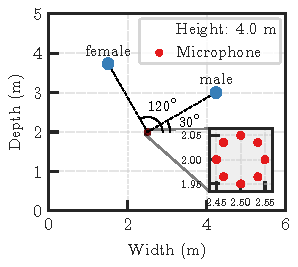
\includegraphics{figures/room_layout.pdf}
  \caption{Room layout.}%
  \label{fig:layout}
\end{figure}

\subsection{Preliminary Experiment}
\todo{準備中…}
\begin{itemize}
  \color{red}
  \item 座標変換あり・なしの場合の共分散行列・分離行列の誤差
  \item 実際のマイク回転角度と推定した回転角度に誤差をつけた場合の実験
\end{itemize}

\subsection{Source Separation Performance}

We compared the following four methods:
\begin{description}
  \item[\NaiveIVA] Online AuxIVA described in \cref{subsec:oiva} as a baseline in our experiments. (See \Cref{alg:naive}.)
  \item[\ResetIVA] Re-initialize covariance and demixing matrices after the CMA rotation CMA. (See \Cref{alg:reset}.)
  \item[\RTObs] Apply SFI for observed signals after the CMA rotation CMA frame by frame. (See \Cref{alg:rtobs}.)
    % \\ $\Obs _{\ft} = \rotMat ^{\hermite} (\rotSpat _{\tframe}) \rot{\Obs} _{\ft}$
  \item[\RTCov] Apply parameter transformation for covariance and demixing matrices after CMA rotation.  (See \Cref{alg:rtcov}.)
    % \\ $\rot{\Demix} _{\ft} \gets \Demix _{\ft} \rotMat ^{\hermite} (\rotSpat _{\tframe})$,\; $\rot{\cov} _{\src,\ft} \gets \rotMat (\rotSpat _{\tframe}) \cov _{\src,\ft} \rotMat ^{\hermite} (\rotSpat _{\tframe})$
\end{description}

The initial values for demixing and covariance matrices were
$\Demix _{\freq,0} = \Eye\; (\forall \freq)$, $\cov _{\src,\freq,0} = 10^{-3}\times\Eye\; (\forall \src, \freq)$, respectively.
We set the number of iteration in each time frame in \cref{alg:naive} $\Itr$ to 5.
We ran experiments with varying forgetting factors $\forget = 0.9, 0.95, 0.98, 0.99$, which were chosen so that the approximate number of frames $\frac{1}{1 - \forget} = 10, 20, 50, 100$.
To increase numerous stability for implementation of online AuxIVA,
we applied the following ad-hoc normalization $\cov _{\src,\ft} \gets \cov _{\src,\ft} + 10 ^{-3} \Eye$ after updates by \eqref{eq:cov}.

\Cref{fig:plots:sisdr} shows the SI-SDRi every \SI{1}{\second}.
Overall, \NaiveIVA{} and \ResetIVA{} showed a significant performance drop after the CMA rotation and improved again with time.
Notably, \ResetIVA{} has the lowest performance before CMA rotaion among all forgetting factors, which gets worse as the forgetting factor approaches 1.
In contrast, proposed \RTCov{} and \RTObs{} methods maintained performance even after the CMA rotation.
Comparing \RTCov{} and \RTObs{}, \RTCov{} performed slightly better.
This may be due to the fact that \RTObs{} estimates the source image at the reference microphone, while the reference signal for SI-SDR evaluation was the source image at the reference position.
\begin{figure}[t]
  \begin{minipage}[t]{\linewidth}
    \centering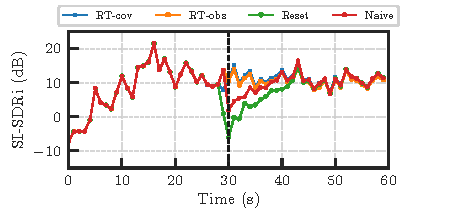
\includegraphics{figures/plots/online/Gauss_8000_fft4096_900.pdf}\subcaption{$\forget = 0.90 $}\label{fig:plot:gauss:900}
    \centering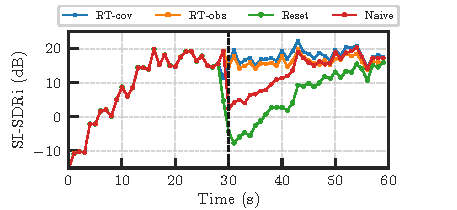
\includegraphics{figures/plots/online/Gauss_8000_fft4096_950.pdf}\subcaption{$\forget = 0.95 $}\label{fig:plot:gauss:950}
    \centering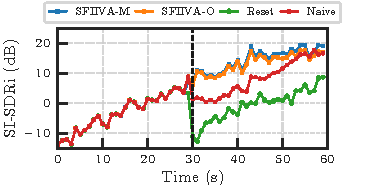
\includegraphics{figures/plots/online/Gauss_8000_fft4096_980.pdf}\subcaption{$\forget = 0.98 $}\label{fig:plot:gauss:980}
    \centering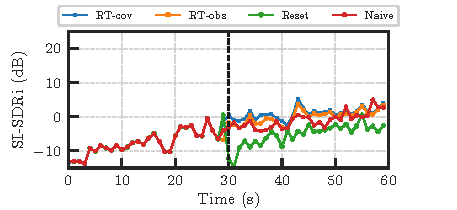
\includegraphics{figures/plots/online/Gauss_8000_fft4096_990.pdf}\subcaption{$\forget = 0.99 $}\label{fig:plot:gauss:990}
    % \centering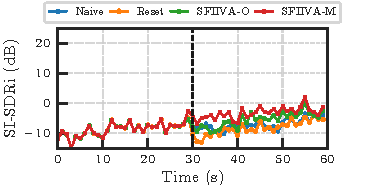
\includegraphics{figures/plots/online/Gauss_8000_fft4096_995.pdf}\subcaption{$\forget = 0.995$}\label{fig:plot:gauss:995}
  \end{minipage}
  \caption{Segmental SI-SDR improvements (SI-SDRi) every \SI{1}{\second} with $\Src = 5$ and $\text{RT}_{60} \approx \SI{100}{\milli\second}$.}%
  \label{fig:plots:sisdr}
\end{figure}

\begin{algorithm}{Online AuxIVA with reset (\textbf{Reset})}{reset}
  \begin{pseudo}
    for $\tframe = 1,\, \dots,\, \rotFra - 1$ \\+
      $\{\Demix _{\ft}\}_{\freq},\, \{\cov _{\src,\ft}\} _{\src,\freq} \gets$ \pr{OIVA}(\{\Obs _{\ft}\} _{\freq}, \{\Demix _{\ft[-1]}\}_{\freq},\, \{\cov _{\src,\ft[-1]}\} _{\src,\freq}) \\-
    {$\Demix _{\freq,\rotFra - 1}$} $\gets$ $\Eye$ \ct{$(\forall \freq)$} \\
    {$\cov _{\src,\freq,\rotFra - 1}$} $\gets$ $\varepsilon \Eye$ \ct{$(\forall \src,\freq)$} \\
    for $\tframe = \rotFra,\, \dots,\, \Tframe$ \\+
      $\{\Demix _{\ft}\}_{\freq},\, \{\cov _{\src,\ft}\} _{\src,\freq} \gets$ \pr{OIVA}(\{\Obs _{\ft}\} _{\freq}, \{\Demix _{\ft[-1]}\}_{\freq},\, \{\cov _{\src,\ft[-1]}\} _{\src,\freq})
  \end{pseudo}
\end{algorithm}

\subsection{Online Rotation Angle Estimation Performance}
\todo{準備中…}

\section{Conclusion}\label{sec:conclusion}
% 本研究では,円状等間隔マイクロホンアレイにおける音場補間をブラインド音源分離に応用した.
% シミュレーション実験により,音場補間が円状等間隔マイクロホンアレイの回転に対するOIVAの頑健性を改善させたことを確認した.
% 今後は本手法の自己回転角度推定 \cite{Lian:2021:APSIPA} との組み合わせや,実時間処理への拡張などに取り組む.
In this study, sound field interpolation for an equally spaced circular microphone array (CMA) was applied to online auxiliary-function-based independent vector analysis (OIVA).
Simulation experiments have confirmed that sound field interpolation improved robustness of OIVA against the rotation of CMA.
Future work includes combining this method with self-rotation angle estimation \cite{Lian:2021:APSIPA} and extending it to real-time processing.

\section*{Biographies}

\noindent\normalsize\textbf{Taishi Nakashima}
received his B.E. in Engineering from Osaka University, Osaka, Japan, in 2019 and his M.S. in Informatics from Tokyo Metropolitan University, Tokyo, Japan, in 2021.
He is pursuing a Ph.D. at Tokyo Metropolitan University and is also a recipient of the JSPS Research Fellowship (DC1) from April 2021.
He is an esteemed Student Member of the Acoustical Society of Japan (ASJ) and the IEEE Signal Processing Society (SPS).
He received the 24th Best Student Presentation Award of ASJ and the 16th IEEE SPS Japan Student Conference Paper Award in 2022, and Top 3\% Recognition at ICASSP 2023.
His research interests primarily focus on blind source separation and acoustic signal processing.
\\

\noindent\normalsize\textbf{Yukoh Wakabayashi}
received the B.E. and M.E. degrees from Osaka University, Osaka, Japan, in 2008 and 2010, respectively, and Ph.D. degree from Ritsumeikan University, Shiga, Japan, in 2017.
He joined Rohm, Inc., Kyoto, Japan, in 2010, and was an assistant researcher with Kyoto University from 2012 to 2014.
He was a recipient of the JSPS Research Fellowship for Young Scientists DC2 from 2016 to 2017.
He was an affiliate assistant professor with Ritsumeikan University from 2018 to 2020.
He is currently an assistant professor with the Department of Computer Science and Engineering, Toyohashi University of Technology, Aichi, Japan, and the Faculty of Systems Design, Tokyo Metropolitan University, Tokyo, Japan.
His research interests include acoustic signal processing, speech phase processing, array signal processing, and speaker diarization.
He is a member of the Institute of Electrical and Electronics Engineers, the Institute of Electronics, Information and Communication Engineers, and Acoustical Society of Japan.
\\

\noindent\normalsize\textbf{Nobutaka Ono}
received his B.E., M.S., and Ph.D. degrees from the University of Tokyo, Japan, in 1996, 1998, and 2001, respectively.
He became a research associate in 2001 and a lecturer in 2005 at the University of Tokyo.
He moved to the National Institute of Informatics in 2011 as an associate professor and then to Tokyo Metropolitan University in 2017 as a full professor.
His research interests include acoustic signal processing, especially microphone array processing, source localization and separation, machine learning, and optimization algorithms.
He is a member of IEEE, EURASIP, APSIPA, IPSJ, IEICE, and ASJ.
He was a member of IEEE Audio and Acoustic Signal Processing (AASP) Technical Committee from 2014 to 2019.
He served as Associate Editor of IEEE Transactions on Audio, Speech, and Language Processing from 2012 to 2015.
He received the best paper award at APSIPA ASC in 2018 and 2021 and Sadaoki Furui Prize Paper Award from APSIPA in 2021.

\printbibliography

\end{document}
